\documentclass[9pt,twocolumn,twoside]{pnas-new}
\usepackage{supertabular}
\usepackage{lscape}
\usepackage{multirow}
\usepackage{tabularx}
\usepackage{csquotes}
\usepackage{upgreek}
\usepackage{hyperref}
% Use the lineno option to display guide line numbers if required.


\templatetype{pnasresearcharticle} % Choose template 

\title{What are we learning from language? Associations between gender biases
and distributional semantics in 25 languages}

% Use letters for affiliations, numbers to show equal authorship (if applicable) and to indicate the corresponding author
\author[a,b,1]{Molly Lewis}
\author[b,1,2]{Gary Lupyan} 

\affil[a]{University of Chicago}
\affil[b]{University of Wisconsin-Madison}

% Please give the surname of the lead author for the running footer
\leadauthor{Lewis} 

% Please add here a significance statement to explain the relevance of your work
\significancestatement{Authors must submit a 120-word maximum statement about the significance of their research paper written at a level understandable to an undergraduate educated scientist outside their field of speciality. The primary goal of the Significance Statement is to explain the relevance of the work in broad context to a broad readership. The Significance Statement appears in the paper itself and is required for all research papers.}

% Please include corresponding author, author contribution and author declaration information
\authorcontributions{Both authors designed research and wrote the paper. M.L. performed research and analyzed the data.}
\authordeclaration{The authors declare no conflict of interest.}
\correspondingauthor{\textsuperscript{2}To whom correspondence should be addressed. E-mail: mollyllewis@gmail.com}

% Keywords are not mandatory, but authors are strongly encouraged to provide them. If provided, please include two to five keywords, separated by the pipe symbol, e.g:
\keywords{distributional semantics $|$ cultural stereotypes $|$ IAT  $|$ gender } 

\begin{abstract}
Cultural stereotypes such as the idea that men are more suited for paid
work while women for taking care of the home and family may contribute
to gender imbalances in STEM fields and other undesirable gender disparities. Here, we test
the hypothesis that word co-occurrence statistics (e.g., the
co-occurrence of ``nurse'' with ``she'') play a causal role in the
formation of the men-career/women-family stereotype. We use word
embedding models to measure bias in the distributional statistics of 25
languages and find that languages with larger biases tend to have
speakers with larger implicit biases (\emph{N} = 657,335). These biases
are further related to the extent that languages mark gender in their
lexical forms (e.g., ``waiter''/``waitress'') hinting that linguistic
biases may be causally related to biases shown in people's implicit
judgments.

\end{abstract}

\dates{This manuscript was compiled on \today}
\doi{\url{www.pnas.org/cgi/doi/10.1073/pnas.XXXXXXXXXX}}

\begin{document}

\maketitle
\thispagestyle{firststyle}
\ifthenelse{\boolean{shortarticle}}{\ifthenelse{\boolean{singlecolumn}}{\abscontentformatted}{\abscontent}}{}

\dropcap{B}y the time they are two, children  have begun to acquire the
gender stereotypes in their culture \cite{gelman2004mother}. These
stereotypes can have undesirable effects. For example, in one study,
6-year-old girls were less likely than boys to choose activities that
were described as for children \enquote{who are very, very smart} and
also less likely to think of themselves as \enquote{brilliant}  \cite{bian2017gender} . Such beliefs may, over time, translate to the
observed lower rates of female participation in STEM fields \cite{ceci2011understanding,leslie2015expectations,miller2015women,stoet2018gender}. For this reason among others,
it is important to better understand how cultural stereotypes are
formed.

A number of recent studies have sought to understand the emergence of structural inequality by studying differences in psychological properties of individuals, such as  such as feelings of self-efficacy in science \cite{stoet2018gender} and general gender preferences \cite{falk2018relationship}.  But, critically, these previous efforts have taken psychological properties individuals as pre-determined, or exogeneous, variables in trying to account for structural inequality. Here, we ask why individuals come to have different feelings and preferences, and argue that language experience plays an important role.

We can distinguish between two major sources of information on which
gender stereotypes may be based. The first is direct experience. For
example, one may observe that most nurses are women and most
philosophers are men and conclude that women are better suited for
nursing and men for philosophy. The second is language. Even without any
direct experience with nurses or philosophers, one may learn about their
stereotypical gender from language about nurses and philosophers.
Languages encode gender in multiple ways. These include gender-specific
titles (\enquote{Mr.} vs.\ \enquote{Miss.}), proper names (\enquote{Sam}
vs.\ \enquote{Ashley}), pronouns (\enquote{he} vs. \enquote{she}),
certain job titles (\enquote{waiter} vs.\ \enquote{waitress}), and
higher-order linguistic associations (otherwise gender-neutral words can
become gendered by being associated with explicitly gendered contexts).
Another source of linguistic information comes from sex-based
grammatical gender systems found in approximately 30\% of languages \cite{wals}. For example, in Spanish, the gender of a
nurse must be specified grammatically (\enquote{enfermer\emph{a}} vs.
\enquote{enfermer\emph{o}}).

To the extent that language is a source of information for forming
cultural stereotypes, two people with similar direct experiences, but
different linguistic experiences, may develop different stereotypes.
Some past work hints at people's surprising sensitivity to
stereotype-relevant information delivered through language. Young
children perform worse in a game if they are told that someone of the
opposite gender performed better than they did on a previous round
\cite{rhodes2008preschoolers}, or merely told that the game is associated
with a particular gender \cite{cimpian2012good}. In some
cases, a subtle turn of phrase can influence children's gender-based
generalization \cite{cimpian2011generic,rhodes2018subtle}. For example, Cimpian and Markman found that children
were more likely to infer that a novel skill is stereotypical of a
gender if the skill is introduced with a generic as opposed a
non-generic subject (``{[}Girls are/There is a girl who is{]} really
good at a game called ``gorp''''). Such work shows that in certain
experimental settings, language can influence stereotype formation. We
were interested in whether it actually does, and by what means.

A widely used method for quantifying cultural stereotypes at an
individual level is the \emph{Implicit Association Test} \cite[IAT]{greenwald1998measuring}. Here, we use previously
administered IATs designed to measure a particular type of gender
stereotype: A bias to associate men with careers and women with family
\cite[\emph{N} = 657,335]{nosek2002harvesting}. These data span native
speakers of 25 languages allowing us to assess how performance varies
with properties of languages. 

Discovering that gender biases in language are correlated with people’s implicit gender biases can be interpreted in at least two ways.  The first is that some cultures have stronger stereotypes and these are reflected in what people talk
about. Language, on this view, simply \emph{reflects} pre-existing
biases. We refer to this as the \emph{language as reflection}
hypothesis. However, language may not simply reflect pre-existing
biases, but may also provide a distinct source of information for
learning about these stereotypes. We refer to this second possibility
that language exerts a causal influence on people's biases as the
\emph{language as causal factor} hypothesis.

In Study 1, we examine whether language-derived gender biases predict
responses on the gender-career IAT. Our analysis focuses on the
\emph{distributional} structure of language rather than the specifics of
the communicated content. In Study 2, we examine how the psychological
biases measured by the IAT and the linguistic biases we measure relate
to more structural aspects of language: sex-based grammatical gender and
the prevalence of gender-specific occupation terms (e.g.,
\enquote{waiter}/\enquote{waitress} but
\enquote{teacher}/\enquote{teacher}). The results of Study 2 suggest
that language not only reflects existing gender biases, but may play a
causal role in shaping them.

\section*{Description of Cross-Cultural Dataset of Psychological Gender
Bias}\label{description-of-cross-cultural-dataset-of-psychological-gender-bias}

Do the implicit and explicit biases measured by the Project Implicit
dataset predict any real world outcomes? We compared our residual
country-level implicit and explicit gender biases to a gender equality
metric reported by the United Nations Educational, Scientific and
Cultural Organization (UNESCO) for each country: the percentage of women
among STEM graduates in tertiary education from 2012 to 2017 \cite{miller2015women,stoet2018gender}. These data were available for 33 out
of 39 of the countries in our sample. Consistent with previous research
(Miller et al., 2015), we found that implicit gender bias was negatively
correlated with percentage of women in STEM fields: Countries with
smaller gender biases tended to have more women in STEM fields (\emph{r}
= -0.54, \emph{p} \textless{} .001). In contrast, there was no
relationship between the percentage of women in STEM fields and the
explicit gender bias measure used by Project Implicit (\emph{r} = 0.14,
\emph{p} = 0.43). In addition, we found a strong correlation between the
median age of each country's population (as reported by the CIA
factbook, 2017) and the residual implicit bias (in which participant age
was held constant): Countries with older populations tended to have
larger gender biases (\emph{r} = 0.64, \emph{p} \textless{} .0001).


Replicating previous analyses \cite{nosek2002harvesting}, older participants showed a greater implicit bias  (\emph{r} = 0.06, \emph{p} \textless{} .0001).  The implicit bias was stronger for female participants (\emph{M} = 0.41, \emph{SD} = 0.35)  than male participants
(\emph{M} = 0.32, \emph{SD} = 0.37; \emph{t} = 96.82, \emph{p}
\textless{} .0001) Implicit bias scores were larger for participants that received the block of trials with bias-incongruent mappings first
relative to the opposite order (\emph{t} = -104.03, \emph{p} \textless{}
.0001).



In sum, we replicate previously-reported patterns of gender bias in the
gender-career IAT literature, with roughly comparable effect sizes \cite[c.f.]{nosek2002harvesting}.
The weak correlation between implicit and
explicit measures is consistent with claims that these two measures tap
into different cognitive constructs \cite{forscher2016meta}. In
addition, we find that implicit gender bias predicts an objective measure of gender equality---female
enrollment in STEM fields. The
finding that older participants show stronger biases may stem from a
cohort effect, but it is not obvious why there is a strong positive
association between the median age of a country's population and a
larger implicit bias when adjusting for the age of individual
participants.

\section*{Study 1: Relating biases in distributional semantics and
human
behavior}\label{study-1-relating-gender-biases-in-distributional-semantics-and-human-behavior}

Are participants' gender biases predictable from the language they
speak? Both the language-as-reflection and language-as-causal-factor
hypotheses predict a positive correlation between the two, but showing
that such a relationship exists is the first step to investigating a
possible causal link. We begin by validating word embedding measures of
gender bias by comparing them to explicit human judgments of word
genderness (Study 1a). We then apply this method to models trained on
text in other languages (Study 1b and 1c). We find that the implicit gender
bias of participants in a country is correlated with the gender bias in
the language spoken in that country.



\begin{figure}
\centering
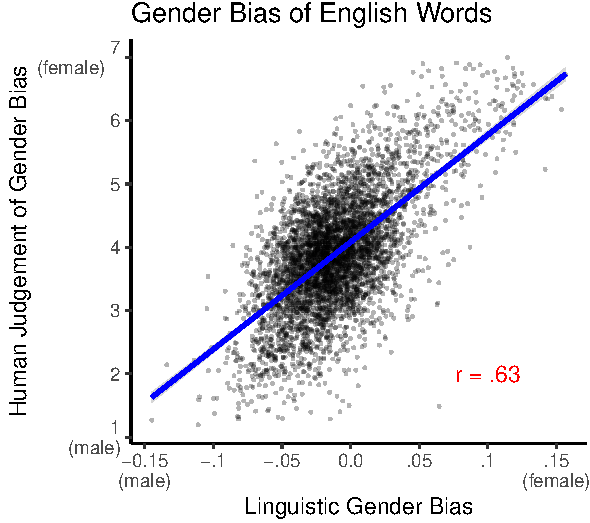
\includegraphics[width=.8\linewidth]{pnas_rmd/iat_lang_pnas_files/figure-latex/unnamed-chunk-10-1.pdf}
\caption{\label{fig:unnamed-chunk-10}Human judgements of word gender bias as
a function of gender bias from the Subtitle-trained embedding model
(Study 1a). Each point corresponds to a word. Larger numbers indicate
stronger association with females (note that this differs from the
design of the rating task, but is changed here for consistency with
other plots). Blue line shows linear fit and the error band indicates
standard error.}
\end{figure}

Estimates of gender bias from the Subtitle corpus (\emph{M} = 0.01;
\emph{SD} = 0.03) and the Wikipedia corpus (\emph{M} = 0; \emph{SD} =
0.03) were highly correlated with each other (\emph{r} = 0.71; \emph{p}
\textless{} .0001). Critically, bias estimates from both word embedding
models were also highly correlated with human judgements (\emph{M} =
4.10; \emph{SD} = 0.92; \emph{r}\textsubscript{Subtitle} = 0.63;
\emph{p} \textless{} .0001; \emph{r}\textsubscript{Wikipedia} = 0.59;
\emph{p} \textless{} .0001; Fig. 1). This suggests that the
psychological gender bias of a word can be reasonably estimated from
word embeddings.

Having validated our method, we now use it to examine the relationship
between psychological and linguistic gender biases. In Study 1b, we
estimate the magnitude of the linguistic bias in the dominant language
spoken in each country represented in the Project Implicit dataset, and
compare this estimate to estimates of psychological gender bias from the
Project Implicit participants.


\begin{figure*}[t!]
\centering
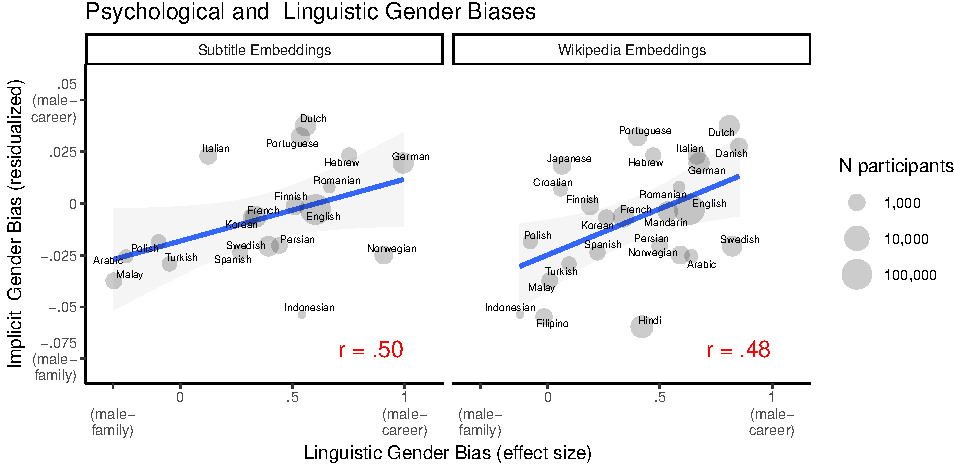
\includegraphics{pnas_rmd/iat_lang_pnas_files/figure-latex/unnamed-chunk-11-1.pdf}
\caption{\label{fig:unnamed-chunk-11}Implicit gender bias (adjusted for participant age,
gender, and block order) as a function of the linguistic gender bias
derived from word-embeddings (Study 1b). Each point corresponds to a
language, with the size of the point corresponding to the number of
participants speaking that language. Linguistic biases are estimated
from models trained on text in each language from Subtitle (left) and
Wikipedia (right) corpora. Larger values indicate a larger bias to
associate men with the concept of career and women with the concept of
family. Error bands indicate standard error of the linear model
estimate.}
\end{figure*}

Despite the differences in the specific content conveyed by the
Subtitles and Wikipedia corpus, the estimated gender bias for each
language was similar across the two corpora (\emph{t}(19) = -0.06,
\emph{p} = 0.95). We next examined the relationship between these
estimates of gender bias for each language and the mean IAT bias score
for participants from countries where that language was dominant (and,
we assume, was the native language of most of these individuals).
Implicit gender bias was positively correlated with estimates of
language bias from both the Subtitle (\emph{r} = 0.5, \emph{p} = 0.02)
and Wikipedia trained models (\emph{r} = 0.48, \emph{p} = 0.01; Fig. 2;
Table 1 shows the language-level correlations between all variables in
Studies 1b and 2). The relationship between implicit gender bias and
language bias remained reliable after partialling out the effect of
median country age (Subtitle: \emph{r} = 0.42, \emph{p} = 0.04;
Wikipedia: \emph{r} = 0.43, \emph{p} = 0.04). Linguistic gender bias was
not correlated with explicit gender bias (Subtitle: \emph{r} = -0.08,
\emph{p} = 0.74; Wikipedia: \emph{r} = 0.34, \emph{p} = 0.09). Estimates
of language bias from the Subtitle corpus were correlated with the
objective measure of gender equality, percentage of women in STEM fields
(\emph{r} = -0.55, \emph{p} = 0.02); this relationship was not reliable
for the Wikipedia corpus (\emph{r} = -0.19, \emph{p} = 0.4).

\begingroup\fontsize{4}{5}\selectfont
\setlength\tabcolsep{1.7pt} % default value: 6pt

\bottomcaption{\label{tab:bigtable}Correlation (Pearson's r) for all measures in Study 1 and 2 at the level of languages. Top panel shows simple correlations; bottom panel shows partial correlations controlling for median country age. Single asterisks indicate \emph{p}  < .05 and double asterisks indicate \emph{p} < .01. The + symbol indicates a marginally significant p-value, \emph{p}  < .1.}
\begin{supertabular}{rlllllllll}




\rotatebox{90}{ } & \rotatebox{90}{Residualized Explicit Bias} & \rotatebox{90}{Residualized Implicit Bias (IAT)} & \rotatebox{90}{Percent Women in STEM} & \rotatebox{90}{Language IAT (Subtitle)} & \rotatebox{90}{Language IAT (Wikipedia)} & \rotatebox{90}{Prop. Gendered Occupation Labels} & \rotatebox{90}{Occupation Bias (Subtitle)} & \rotatebox{90}{Occupation Bias (Wikipedia)} & \rotatebox{90}{Median Country Age}\\
\midrule
\addlinespace[0.3em]
\multicolumn{10}{l}{\textbf{Simple Correlations}}\\
\hspace{1em}Residualized Explicit Bias &  & \ .18 & \ .18 & -.08 & \ .34+ & \ .11 & \ .28 & \ .29 & -.07\\
\hspace{1em}Residualized Implicit Bias (IAT) & \ .18 &  & -.53* & \ .50* & \ .48* & \ .57** & \ .64** & \ .59** & \ .61**\\
\hspace{1em}Percent Women in STEM & \ .18 & -.53* &  & -.55* & -.19 & -.35 & -.39 & -.32 & -.42+\\
\hspace{1em}Language IAT (Subtitle) & -.08 & \ .50* & -.55* &  & \ .51* & \ .28 & \ .42+ & \ .40+ & \ .31\\
\hspace{1em}Language IAT (Wikipedia) & \ .34+ & \ .48* & -.19 & \ .51* &  & \ .18 & \ .28 & \ .44* & \ .25\\
\hspace{1em}Prop. Gendered Occupation Labels & \ .11 & \ .57** & -.35 & \ .28 & \ .18 &  & \ .75** & \ .70** & \ .35+\\
\hspace{1em}Occupation Bias (Subtitle) & \ .28 & \ .64** & -.39 & \ .42+ & \ .28 & \ .75** &  & \ .80** & \ .36\\
\hspace{1em}Occupation Bias (Wikipedia) & \ .29 & \ .59** & -.32 & \ .40+ & \ .44* & \ .70** & \ .80** &  & \ .34+\\
\hspace{1em}Median Country Age & -.07 & \ .61** & -.42+ & \ .31 & \ .25 & \ .35+ & \ .36 & \ .34+ & \\
\addlinespace[0.3em]
\multicolumn{10}{l}{\textbf{Partial Correlations}}\\
\hspace{1em}Residualized Explicit Bias &  & \ .28 & \ .16 & -.06 & \ .38+ & \ .14 & \ .33 & \ .34 & \\
\hspace{1em}Residualized Implicit Bias (IAT) & \ .28 &  & -.38+ & \ .42* & \ .43* & \ .48* & \ .57** & \ .52** & \\
\hspace{1em}Percent Women in STEM & \ .16 & -.38+ &  & -.49* & -.09 & -.23 & -.28 & -.20 & \\
\hspace{1em}Language IAT (Subtitle) & -.06 & \ .42* & -.49* &  & \ .47* & \ .20 & \ .35+ & \ .33 & \\
\hspace{1em}Language IAT (Wikipedia) & \ .38+ & \ .43* & -.09 & \ .47* &  & \ .11 & \ .21 & \ .39+ & \\
\hspace{1em}Prop. Gendered Occupation Labels & \ .14 & \ .48* & -.23 & \ .20 & \ .11 &  & \ .71** & \ .66** & \\
\hspace{1em}Occupation Bias (Subtitle) & \ .33 & \ .57** & -.28 & \ .35+ & \ .21 & \ .71** &  & \ .77** & \\
\hspace{1em}Occupation Bias (Wikipedia) & \ .34 & \ .52** & -.20 & \ .33 & \ .39+ & \ .66** & \ .77** &  & \\
\bottomrule
\end{supertabular}

\endgroup{}

In Study 1c, we conducted a confirmatory, pre-registered analysis of our hypothesis that biases present in language statistics are reflected in the psychological biases of speakers of those languages. We leveraged the Attitudes, Identities, and Individual Differences Study dataset \cite[AIID]{aiid} containing measures of IAT performance from over 200,000 participants for a wide range of IATs (e.g. career - family, team - individual, etc.). All the tests were conducted using English words and most participants were English speakers. The dataset allowed us to compare biases between participants who spoke two different dialects of English: British and American. For each of the 31 IATs in the sample, we predicted that the degree to which that bias was present in a speaker’s English dialect (British or American) would predict the magnitude of their psychological bias, as measured by the IAT.

Figure 3 visualizes the critical interaction term. Behavioral performance on the different IATs was correlated with language statistics. When language statistics predicted that US-English had a greater bias, American participants showed a greater bias. When language statistics predicted that UK-English had a greater bias, British participants showed a greater bias (\(\beta\) = -.05, \emph{SE} = .02, \emph{t} = -2.88; see SI for full model results).

\begin{figure}
\centering
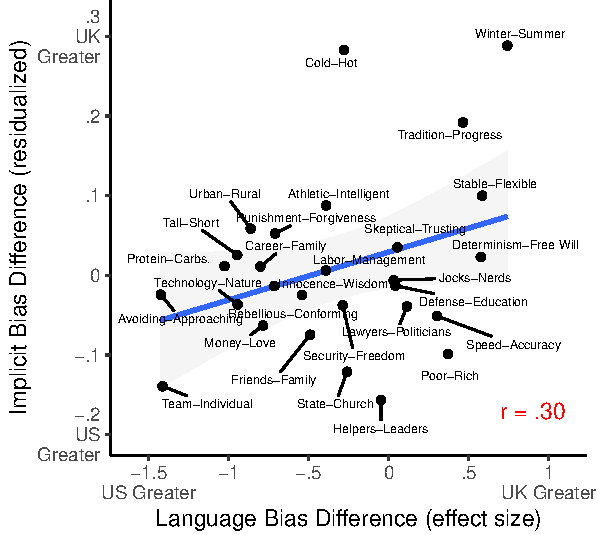
\includegraphics[width=.8\linewidth]{pnas_rmd/iat_lang_pnas_files/figure-latex/1cplot-1.pdf}
\caption{\label{fig:1cplot}Difference (UK minus US) in implicit bias
versus linguistic bias for 31 IAT types.}
\end{figure}

In Study 1, we found that a previously-reported psychological gender bias – the bias to associate men with career and women with family – was correlated with the magnitude of that same bias as measured in the language statistics of 25 languages. Participants completing the IAT in countries where the dominant language had stronger associations between men and career words, and women and family words, showed stronger biases on the gender-career IAT. In a pre-registered, confirmatory analysis, we also find that this pattern extends to biases beyond associating males with career and women with family: In a comparison of 31 different IATs, the magnitude of the bias in speaker’s dialect of English (US vs. UK) predicted their behavioral bias, as measured by the IAT. These results are consistent with both the \emph{language-as-reflection} and
\emph{language-as-causal-factor} hypotheses. In Study 2, we try to
better distinguish between these hypotheses by investigating whether the
gender-career bias is associated with two structural features of
language: grammatical gender and the presence of gendered occupation
terms (e.g., waiter/waitress). In Study 2 we try to distinguish between these hypotheses.

\section*{Study 2: Gender bias and lexicalized
gender}\label{study-2-gender-bias-and-lexicalized-gender}

The association between language bias and implicit bias is predicted by both the language-as-reflection and language-as-causal-factor hypotheses, but for different reasons. If language is causally related to implicit biases, then differences in the structural aspects of language that act to exaggerate linguistic gender bias should predict greater implicit bias. This relationship is not predicted by the language-as-reflection hypothesis.

 One such structural difference concerns the
grammaticalization of gender. Some languages such as Spanish mark gender
distinctions in a grammatically obligatory way, e.g.,
\enquote{enfermero} (nurse-\textsc{masc}) versus \enquote{enfermera}
(nurse-\textsc{fem}). Grammatical gender systems frequently demand
gender-based agreement, e.g., \enquote{el enfermero alto} (the tall
nurse-\textsc{masc}) versus \enquote{la enfermera alta} (the tall
nurse-\textsc{fem}), which while informationally redundant, may act to
amplify gender biases in the language. Another structural difference is the existence of gender-specific terms such as  \enquote{waiter} vs.
\enquote{waitress}, which are more frequent in some languages than others.  Languages with grammatical gender do tend to use
more such terms, but the two are distinct. French has grammatical
gender, but many occupation terms are gender-neutral (e.g., auteur,
athlète, juge).

In Study 2, we examined whether grammatical gender and use of
gender-specific occupation terms are associated with a greater
psychological gender bias and whether this relationship is further
mediated by language statistics. Finding such associations would lend support to the language-as-causal-factor hypothesis because grammatical gender and (to a somewhat lesser degree) lexical gender encoding are relatively stable features of language. Although both can change over time, these changes are largely independent of the propositional content conveyed by language. For example, a Finnish document about nursing being unsuitable for men would still use a gender-neutral form of
\enquote{nurse} while a Spanish document promoting nursing careers to
men would be committed to using gender-marked forms.




\begin{figure}
\centering
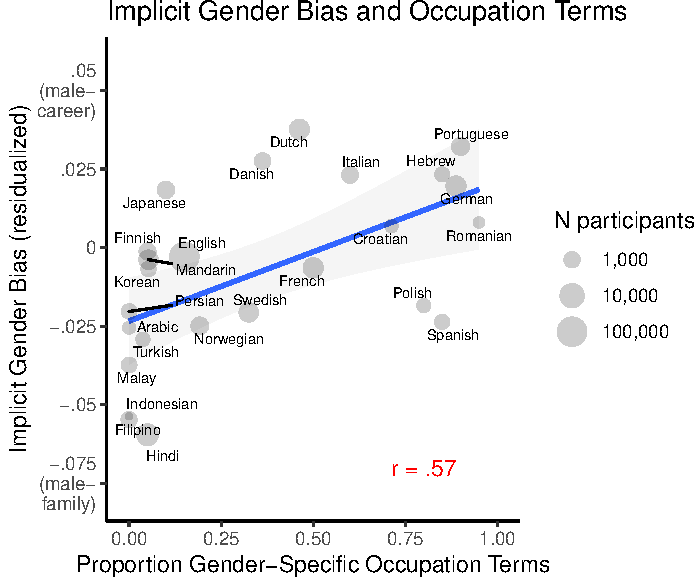
\includegraphics[width=.8\linewidth]{pnas_rmd/iat_lang_pnas_files/figure-latex/unnamed-chunk-14-1.pdf}
\caption{\label{fig:unnamed-chunk-14}Implicit gender bias (adjusted for participant age,
gender, and block order) as a function of the proportion of gender-specific
labels for set of words referring to occupations. Each point corresponds
to a language, with the size of the point corresponding the number of
participants speaking that language. Error band indicates standard error
of the linear model estimate.}
\end{figure}

In additive linear models controlling for median country age, there was
no difference in implicit or explicit psychological gender bias for
speakers of languages with a grammatical gender system (\emph{N} = 12),
compared to those without (\emph{N} = 13; Implicit: \(\beta\) = 0;
\emph{SE} = 0.01; \emph{t} = -0.43; Explicit: \(\beta\) = -0.09;
\emph{SE} = 0.07; \emph{t} = -1.23).  Implicit gender
bias was reliably correlated with degree of gender-specific marking on
occupation words: Languages with more gender-specific forms tended to
have speakers with greater psychological gender bias (\emph{r} = 0.57,
\emph{p} \textless{} .01; Fig.\ 4). This relationship remained after partialling out the effect of
median country age (\emph{r} = 0.48, \emph{p} = 0.02; Table 1). There
was no relationship between explicit psychological gender bias and
lexical marking of occupation words after partialling out the effect of
median country age (\emph{r} = 0.14, \emph{p} = 0.51).

\begin{figure*}[t!]
\centering
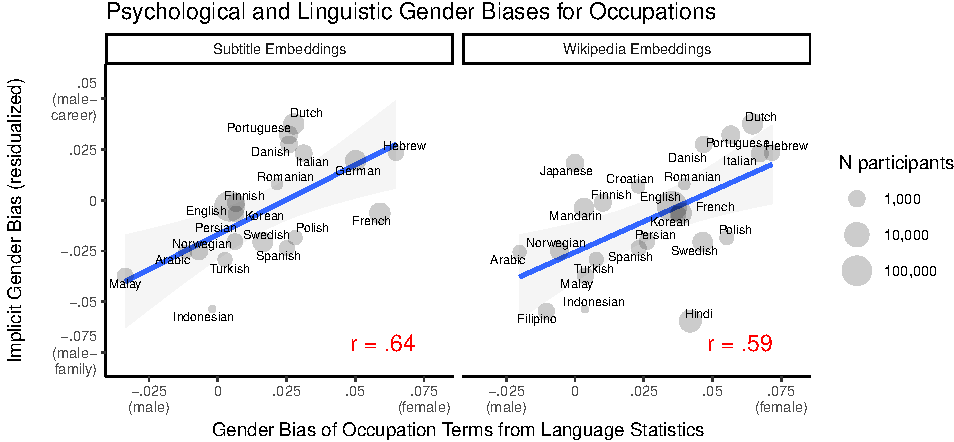
\includegraphics{pnas_rmd/iat_lang_pnas_files/figure-latex/unnamed-chunk-15-1.pdf}
\caption{\label{fig:unnamed-chunk-15}Implicit gender bias (adjusted for participant age,
gender, and block order) as a function of mean gender bias of words
referring to occupations, with each point corresponding to a language
(Study 2). The size of the point corresponds the number of participants
speaking that language. Occupation gender bias is estimated for each
language from word embedding models trained on Subtitle (left) and
Wikipedia (right) corpora. Error bands indicate standard error of the
linear model estimate.}
\end{figure*}

We next examined whether the existence of gender-specific occupation terms was associated with a greater encoding of gender bias in the language. We fit a mixed effects model predicting degree of gender bias in language statistics (estimated from word embedding models) from distinctiveness between male and female forms for that word, with random intercepts and slopes by language. Having more distinct occupation terms was associated with greater linguistic gender bias for those occupations. This was true for models trained on both the Subtitle corpus (\(\beta\) = 0.59; \emph{SE} = 0.07; \emph{t} = 8.72) and Wikipedia
corpus (\(\beta\) = 0.81; \emph{SE} = 0.09; \emph{t} = 9.48). For example, \enquote{secretary} had greater gender bias in Italian, which has distinct male and female terms, compared to English, which has only one term. 

This relationship also held at the level of languages: Languages with more
distinct forms had a greater bias in language statistics
(Subtitle: \emph{r} = 0.75, \emph{p} \textless{} .01; Wikipedia:
\emph{r} = 0.7, \emph{p} \textless{} .01; i.e., Italian has greater overall gender bias compared to English).

Finally, we examined the relationship between gender bias in language
statistics and psychological gender biases at the level of languages.
Unlike in Study 1, all the target words in the present study referred to
people (occupations) and thus potentially could be marked for the gender
of the referenced person. Consequently, if explicit gender marking
drives language statistics, we should expect to see a strong positive
relationship at the level of languages between bias in language
statistics \emph{for occupation words} and psychological biases for
speakers of that language. Consistent with this prediction, gender bias
in language statistics for occupation words was positively correlated
with implicit gender bias (Subtitle: \emph{r} = 0.64, \emph{p}
\textless{} .01; Wikipedia: \emph{r} = 0.59, \emph{p} \textless{} .01),
and remained reliable after partialling out the effect of median country
age (Subtitle: \emph{r} = 0.57, \emph{p} \textless{} .01; Wikipedia:
\emph{r} = 0.52, \emph{p} = 0.01; Fig. 5). In contrast,  explicit psychological gender bias was not predicted by language statistics, even after partialling out the effect of median country age (Subtitle: \emph{r} = 0.33, \emph{p} = 0.12;
Wikipedia: \emph{r} = 0.34, \emph{p} = 0.11).

To understand the relative predictive power of language statistics and
distinct occupation terms, we fit an additive linear model predicting implicit bias
from language statistics and proportion distinct forms, controlling for
median country age. Because language statistics for occupation terms and
proportion distinct forms were highly colinear (Wikipedia: \emph{r} =
0.70, \emph{p} \textless{} .001; Subtitle: \emph{r} = 0.75, \emph{p}
\textless{} .001), we used the estimate of bias in language statistics
for each language based on the set IAT words described in Study 1b. Both
gender bias in language statistics (based on IAT words) and the
proportion of gender-specific occupation titles were independent
predictors of implicit bias. The two predictors accounted for 49\% of
variance in implicit bias when using the Subtitle corpus and 60\% of
variance for the Wikipedia corpus. Full model results are reported in
the SI.

The strong collinearity between language statistics for
occupation terms and proportion gender-specific occupations forms is
consistent with a causal model in which language statistics mediate the
effect of gender-specific forms on implicit bias: The presence of
distinct forms referring to people of different genders \emph{leads to}
biased language statistics, which in turn leads to gender bias in
behavior. Consistent with this model, a bootstrap test of mediation
revealed a marginal effect for the Subtitle model (path-ab = 0.28,
\emph{p} = 0.10; Alfons, 2018), and significant mediation effect for the
Wikipedia model (path-ab = 0.35, \emph{p} =
0.04).\footnote{Though our power to detect this effect is relatively low \cite[approximately, .4]{schoemann2017determining}.}

In Study 2, we asked whether structural features of language -- the
presence of a grammatical gender systems and the propensity to
lexicalize gender distinctions -- correlated with implicit bias.
Grammatical gender was not reliably correlated with implicit bias.
Languages that use more gender-specific occupation terms, however did
predict a greater implicit bias. There is some evidence that the effect
of lexical gender distinctions on implicit bias may be mediated by the
influence this terminology introduces on the ways that gender is
statistically encoded in different language. What does this finding mean
for our two hypotheses? The fact that, e.g., German explicitly marks the
gender of professors while English does not, has cognitive consequences
for German speakers; it is not simply a matter of current cultural
differences being reflected in language. Language does not merely
reflect our biases, it seems to contribute to them.

\section*{Discussion}\label{general-discussion}

Where do we get our gender stereotypes? Non-linguistic experiences surely play a role, but might we also be learning our biases from the statistics of language to which we are exposed? We used a large-scale dataset of Implicit Association Tests (IATs) measuring the bias to associate men with career and women with family and related people’s measured implicit bias to the statistics of the dominant language spoken in the country of the participants. In Study 1, we found that languages with a greater gender bias in their distributional structure, tend to have speakers that have stronger implicit biases. In Study 2, we found a positive relationship between a structural language feature – the prevalence of gender-marked occupation terms – and implicit bias. There is suggestive evidence that this greater implicit bias is mediated by the greater gender bias encoded in the distributional patterns of gender-marked terms.

Our work is the first to characterize the relationship between broad structural patterns in language and cultural stereotypes. The positive correlation between gender bias in language and gender bias in speakers is consistent both with language playing a causal role in the emergence of cultural stereotypes and the idea that language merely reflects existing stereotypes of its speakers. However, the positive association between prevalence of gender-specific terms and implicit bias (Study 2) is most parsimoniously explained by language statistics (partially) causing the observed differences in implicit bias. It is implausible that nonlinguistically acquired gender biases could have changed the lexical inventory of the language rapidly enough to explain the differences in IAT performance that we observed. Future work could use experimental methods to manipulate language statistics in order to more directly examine these causal influences.


Our findings do not contradict previous reports that differences in e.g., STEM participation by men and women are associated with differences in self-efficacy \cite{stoet2018gender} and inherent differences in gender preferences \cite{falk2018relationship}. However, they provide a potential explanation of the origins of these psychological biases by arguing that exposure to biased language statistics could play a causal role in the emergence of these biases at the level of the individual. Consistent with this account, biases in language statistics are correlated with previously reported individual-level predictors of STEM inequality, such as self-efficacy in science and general preferences (see SI for details).

One limitation of our work is the reliance on the IAT, which has been criticized for both its low reliability \cite{lane2007understanding} and limited external validity \cite{fazio2003implicit}. Issues of reliability are less relevant here because we use the IAT to measure group-level differences rather than as an individual-difference measure. However, concerns about validity are important particularly because we find that language measures and explicit psychological measures of gender bias are uncorrelated, though explicit bias was measured in a fairly coarse way. The strong negative correlation we find between the proportion women in STEM and language bias (\emph{r} = -.55) provides compelling evidence that language biases are related to real-world consequences, but understanding the full import of linguistic biases on cultural stereotypes will require obtaining measures more closely related to real-world behavior. 

Cultural stereotypes are acquired through experience. Here, we show that
group-level differences in implicit bias are strongly correlated with
the strength of gender bias encoded in the statistics of different
languages. This pattern suggests that the statistics of language use are
an important source of cultural experience: The mere process of
listening to and producing language exposes one to statistics that may
lead to the formation of cultural stereotypes. Many cultural
associations present in the statistics of language may be innocuous --
indeed, these statistics may be an important mechanism through which
cultural information is transmitted (Lupyan \& Lewis, 2017). But, in
other cases, like the kind of gender stereotypes investigated here,
language may play a powerful role in their formation, and ultimately
contribute to undesirable structural inequality. Understanding the causal role that language plays in the
formation of these stereotypes is therefore an important first step to
changing these consequences.

\matmethods{All data and code are available online (\url{https://github.com/mllewis/IATLANG}). Supplementary Information available at:  \url{https://mollylewis.shinyapps.io/iatlang_SI/}.
\subsection*{Description of IAT dataset}

To quantify cross-cultural gender bias, we used data from a large-scale
administration of an Implicit Association Task \cite[IAT]{greenwald1998measuring} by Project Implicit \cite[\url{https://implicit.harvard.edu/implicit/}]{nosek2002harvesting}. The IAT measures the strength of
respondents' implicit associations between two pairs of concepts (e.g.,
male-career/female-family vs.~male-family/female-career) accessed via
words (e.g., \enquote{man,} \enquote{business}). The underlying
assumption of the IAT is that words denoting more similar meanings
should be easier to pair together compared to more dissimilar pairs.

Meanings are paired in the task by assigning them to the same response
keys in a two-alternative forced-choice categorization task. In the
critical blocks of the task, meanings are assigned to keys in a way that
is either bias-congruent (i.e.~Key A = male/career; Key B =
female/family) or bias-incongruent (i.e.~Key A = male/family; Key B =
female/career). Participants are then presented with a word related to
one of the four concepts and asked to classify it as quickly as possible
(see Study 1b Methods for list of target words). Slower reaction times
in the bias-incongruent blocks relative to the bias-congruent blocks are
interpreted as indicating an implicit association between the
corresponding concepts (i.e.~a bias to associate male with career and
female with family).

We analyzed gender-career IAT scores collected by Project Implicit
between 2005 and 2016, restricting our sample based on participants'
reaction times and error rates using the same criteria described in \cite[pg.~104]{nosek2002harvesting}. We only analyzed data for
countries that had complete demographic information and complete data
from the IAT for least 400 participants (2\% of these respondents did
not give responses to the explicit bias question). This cutoff was
arbitrary, but the pattern of findings reported here holds for a range
of minimum participant values (see
SI). Our final sample included 657,335 participants from 39 countries, with a
median of 1,145 participants per country. Importantly, although the
respondents were from largely non-English speaking countries, the IAT
was conducted in English. We do not have language background data from
the participants, but we assume that a large fraction of the respondents
from non-English speaking countries were native speakers of the dominant
language of the country and second language speakers of English. The fact that the test was administered in English make our analyses conservative, lowering the likelihood of finding language-specific predictors of the kind we report here.

To quantify the strength of participants’ implicit bias as assessed by the IAT we adopt the widely used  \emph{D-score}, which measures the difference between critical blocks for each participant while controlling for individual differences
in response time \cite{greenwald1998measuring}. After completing
the IAT, participants were asked \enquote{How strongly do you associate
the following with males and females?} for both the words
\enquote{career} and \enquote{family.} Participants indicated their
response on a Likert scale ranging from \emph{female} (1) to \emph{male}
(7). An explicit gender-career bias score was defined as their Career response minus their Family response such that greater values indicate a greater bias to associate males with career.


\subsection*{Study 1a}

To model word meanings, we use semantic embeddings derived from a model
that learns meanings by trying to predict a word from surrounding words,
given a large corpus. The core assumption of these models is that the
meaning of a word can be described by the words it tends to co-occur
with---words occurring in similar contexts, tend to have similar
meanings \cite{firth1957synopsis}. A word like \enquote{dog,} for example is
represented as more similar to \enquote{cat} and \enquote{hound} than to
\enquote{banana} because \enquote{dog} co-occurs with words more in
common with \enquote{cat} and \enquote{hound} than with \enquote{banana} \cite{landauer1997solution,lund1996producing}. Recent developments
in machine learning allow the idea of distributional semantics to be
implemented in a way that takes into account many features of language
structure while remaining computationally tractable. The best known of
these word embedding models is \emph{word2vec} \cite{mikolov2013efficient}. By attempting to predict the words that surround another
word, the model is able to learn a vector-based representation for each
word that represents its similarity to other words, i.e., a semantic
embedding. We can then compute the similarity between two words by
taking the distance between their vectors (e.g., cosine of angle).

In order to validate word embeddings as a measure of psychological
gender bias, we used an existing set of word norms in which participants
were asked to rate \enquote{the gender associated with each word} on a
Likert scale ranging from \emph{very feminine} (1) to \emph{very
masculine} \cite[7]{scott2018glasgow}. We
compared these norms to estimates of gender bias obtained from embedding
models pre-trained on two different corpora of English text: Wikipedia
\cite{bojanowski2016enriching} and subtitles from movies
and TV shows \cite{vanparidon,lison}. The Wikipedia corpus is a large, naturalistic corpus of written
language; the Subtitle corpus is a smaller corpus of spoken language.
Both models were trained using the fastText algorithm \cite[a variant of
word2vec]{joulin2016bag}. There were 4,671
words in total that overlapped between the word-embedding models and
human ratings.

Using the word embeddings, we calculated an estimate of gender bias for
each word by measuring the average cosine distance to a standard set of
male \enquote{anchor} words (\enquote{male,} \enquote{man,}
\enquote{he,} \enquote{boy,} \enquote{his,} \enquote{him,}
\enquote{son,} and \enquote{brother}; Nosek, Banaji, \& Greenwald, 2002)
and the average cosine similarity to a set of female words
(\enquote{female,} \enquote{woman,} \enquote{she,} \enquote{girl,}
\enquote{hers,} \enquote{her,} \enquote{daughter,} and
\enquote{sister}). A gender score for each word was then obtained by
taking the difference of the similarity estimates (mean male similarity
- mean female similarity), such that larger values indicated a stronger
association with males.

\subsection*{Study 1b}

Previous work has shown biases studied using IATs can be predicted from
the distributional statistics of language (word co-occurrences). Using
these statistics, Caliskan, Bryson, and Narayanan \cite[henceforth,
CBN]{caliskan2017semantics} measured the distance between the words presented to participants
in the IAT task. CBN found that these distances were highly correlated
with the biases computed by a variety of IATs (e.g., valence and
Caucasian vs.~African-American names; gender and math vs.~arts;
permanence and mental vs.~physical diseases). CBN only measured semantic
biases in English. Here, we extend CBN's method to 25 languages
examining whether languages with a stronger gender bias as expressed in
distributional semantics predict stronger implicit and explicit gender
biases on a large dataset of previously administered gender-career IATs.

We identified the most frequently spoken language in each country in our
analysis using Ethnologue \cite{simons2018}. After exclusions
(see below), our final sample included 25
languages (note that while Hindi is identified as the most frequently spoken language in India, India is highly multilingual and so Hindi embeddings may be a poor representation of  the linguistic statistics for speakers in India as a group).
For each language, we obtained translations from native speakers for the
stimuli in the Project Implicit gender-career IAT behavioral task (Nosek
et al., 2002) with one slight modification. In the behavioral task,
proper names were used to cue the male and female categories
(e.g.~\enquote{John,} \enquote{Amy}), but because there are not direct
translation equivalents of proper names, we instead used a set of
generic gendered words which had been previously used for a different
version of the gender IAT \cite[e.g., ``man,'' ``woman;'']{nosek2002harvesting} . Our linguistic stimuli were therefore a set of 8 female and 8
male Target Words (identical to Study 1a), and the set of 8 Attribute
Words words used in the Project Implicit gender-career IAT: 8 related to
careers (\enquote{career,} \enquote{executive,} \enquote{management,}
\enquote{professional,} \enquote{corporation,} \enquote{salary,}
\enquote{office,} \enquote{business}) and 8 related to families
(\enquote{family,} \enquote{home,} \enquote{parents,}
\enquote{children,} \enquote{cousins,} \enquote{marriage,}
\enquote{wedding,} \enquote{relatives}). For one language, Filipino, we
were unable to obtain translations from a native speaker, and so
Filipino translations were compiled from dictionaries.

We used these translations to calculate a gender bias effect size from
word embedding models trained on text in each language. Our effect size
measure is a standardized difference score of the relative similarity of
the target words to the target attributes (i.e.~relative similarity of
male to career vs.~relative similarity of female to career). Our effect
size measure is identical to that used by CBN with an exception for
grammatically gendered languages (see SI for replication of CBN on our
corpora). Namely, for languages with grammatically gendered Attribute
Words (e.g., niñas for female children in Spanish), we calculated the
relationship between Target Words and Attribute Words of the same gender
(i.e.~\enquote{hombre} (man) to \enquote{niños} and \enquote{mujer}
(woman) to \enquote{niñas}). In cases where there were multiple
translations for a word, we averaged across words such that each of our
target words was associated with a single vector in each language. In
cases where the translation contained multiple words, we used the entry
for the multiword phrase in the model when present, and averaged across
words otherwise. Like the psychological measures of bias from the
Project Implicit data, larger values indicate larger gender bias.

We calculated gender bias estimates using the same word embedding models
as in Study 1a (Subtitle and Wikipedia corpora). We excluded languages
from the analysis for which 20\% or more of the target words were
missing from the model or the model did not exist. This led us to
exclude one language (Zulu) from the analysis of the Wikipedia corpus
and six languages from the analysis of the Subtitle corpus (Chinese,
Croatian, Hindi, Japanese, Filipino, and Zulu). Our final sample
included 25 languages in total (\emph{N}\textsubscript{Wikipedia} = 25;
\emph{N}\textsubscript{Subtitle} = 20), representing 8 language
families. 

We calculated language-level measures for four
additional measures by averaging across countries whose participants
speak the same language: implicit and explicit psychological gender bias
(estimated from the Project Implicit dataset), percentage of women in
STEM fields, and median country age.  To account for the above-mentioned influences on
implicit bias, we calculated a residual implicit bias score for each
participant, controlling for participant age, participant gender, and block
order. We also calculated a residual explicit bias score controlling for
the same set of variables. We then averaged across participants to
estimate the country-level gender bias (Implicit: \emph{M} = -0.01;
\emph{SD} = 0.03; Explicit: \emph{M} = 0.00; \emph{SD} = 0.18). Implicit
gender biases were moderately correlated with explicit gender biases at
the level of participants (\emph{r} = 0.16, \emph{p} \textless{} .0001)
but not countries (\emph{r} = 0.26, \emph{p} = 0.12).



\subsection*{Study 1c}

The AIID datset was partitioned into two samples: exploratory (15\%) and
confirmatory (85\%). Based on the exploratory sample, we pre-registered
our analysis plan for the confirmatory sample
(\url{https://osf.io/3f9ed}) and were given access to the confirmatory dataset only after our pre-registration was approved. 

Of the 95 IATs present in the dataset, we identified 31 types based on the following criteria: (1) stimuli were words rather than pictures, and (2) 75\% of the target words for each IAT test were present in both our US and UK English corpora. To measure linguistic bias, we trained word embedding models on equally-sized subsets of British National Corpus (BNC; Burnard 1995) and Corpus of Contemporary American English (COCA; Davies 2008). The model was trained using the fastText alogrithm \cite{joulin2016bag}, with a vector size of 400 and  window size of 10. We then calculated a language bias effect size for each IAT in each English dialect, using the same method as in Study 1b. 


Within the confirmatory AIID dataset, there were 187,969 administrations
of the IAT. After data exclusion (using criteria similiar to Study 1a; see SI for details), our final sample
included data from 135,240 administrations of the IAT across the 31 IATs (USA: \emph{N} = 127,630; UK: \emph{N} = 7,610). Each participant
completed an average of 6.13 different IATs (\emph{SD} = 3.99). For each administrations of an IAT, we calculated a residual D-score which controlled for participant gender, age, education, task order (whether implicit or explicit measures were completed first), and block order (whether congruent or incongruent mappings occurred first).

We fit a linear mixed effect model predicting the magnitude of the IAT bias for each participant from their location (US vs.\ UK), the linguistic bias from US-English and UK-English trained models, and the interaction of the two factors. We included participant and IAT test as random intercepts. This model differs from the pre-registered analysis, which is also consistent with results of the presented analysis, but does not account for participant-level variance (see SI for results of the exact pre-registered model).


\subsection*{Study 2}

We identified 20 occupation terms that can be translated into  all 25 of our languages, and that were balanced in terms of
their perceived gender bias in the workforce \cite{misersky2014norms}. We
then translated these words into each of the 25 languages in our sample,
distinguishing between male and female variants (e.g., \enquote{waiter}
vs. \enquote{waitress}) where present. The words were translated by
consulting native speakers and dictionaries.

We coded each language for the presence or absence of a sex-based
grammatical gender system using WALS \cite{wals} and
other sources, as necessary. We quantified lexical encoding of gender as the proportion of the 20 occupations within each language for which the male and female forms differed. Larger values indicate a preponderance for more gender-specific forms.  Languages with grammatical gender
systems were more likely to have gender-specific terms for occupations
(\emph{t}(14.89) = 4.85, \emph{p} \textless{} .001). We then estimated the extent to which each occupation term was gender biased in its language statistics using word
embedding models trained in each language on the Subtitle and Wikipedia
corpora. For each occupation term, we estimated its bias in language
statistics using the same pairwise similarity metric as in Study 1a, and
then averaged across occupations within a language to get a
language-level estimate of gender bias. Larger values indicate greater
gender bias in language statistics. We then compared each of the three
language measures (grammatical gender, proportion specific gender forms,
and bias in language statistics for occupation words) to the
psychological gender measures described in Study 1b (implicit and
explicit bias, adjusted for age, gender and block order).

}

\showmatmethods{} % Display the Materials and Methods section

\showacknow{} % Display the acknowledgments section

% Bibliography
\bibliography{library.bib}

\end{document}